
% Chapter 3

\chapter{Results} % 3rd chapter title

\label{Chapter3} % For referencing the chapter elsewhere, use \ref{Chapter3} 

%----------------------------------------------------------------------------------------

%----------------------------------------------------------------------------------------

\section{Presentation of the $\phi$-FEM technique}

\subsection{The Classic FEM approach}
As indicated by its name, the $\phi$-FEM technique is based on the classic FEM technique \parencite[p.111]{ern2013theory}. Let $\Omega$ be a bounded domain in $\mathbb{R}^d$ with a regular boundary $\partial\Omega$. Let $\cal{L}$ be a scalar elliptic operator \parencite{evans}. Given a function $f\ \in L^2(\Omega)$, and another function $g\ \in L^2(\partial \Omega)$, the problem is to solve
\begin{align}
    \begin{cases}
        \mathcal{L} u = f  \quad &\text{in } \Omega \\
        u = g & \text{on } \partial\Omega \,.
    \end{cases}
    \label{eq:problem}
\end{align}
Except for the non-homogeneous Dirichlet case \footnote{The non-homogeneous Dirichlet case can be brought back to the \ref{eq:varForm} by writing $u=u_g + \Phi$, where $u_g$ is a lifting function, and $\Phi$ satisfies \ref{eq:varForm} where $V=H^1_0(\Omega)$}, problems of the form \eqref{eq:problem} can be transformed into a weaker form called variational formulation :
\begin{align}
    \text{Seek } u \in V \text{ such that} \quad a(u,v)=f(v), \quad \forall v \in V \,
    \label{eq:varForm}
\end{align}
where $V$ is a Hilbert space satisfying
\begin{align*}
    H_0^1 (\Omega) \subset V \subset H^1 (\Omega) \,.
\end{align*}
Moreover, $a$ is a bilinear form defined on $V\times V$, and $f$ is a linear form defined on $V$.

The Poisson problem ($\mathcal{L} := -\Delta$) with homogeneous boundary condition is a classic example of an elliptical PDE that can be formulated as in \eqref{eq:varForm}. It is defined as 
\begin{align}
    \begin{cases}
        -\Delta u = f  &\quad \text{in } \Omega \\
        u = 0  &\quad \text{on } \partial\Omega
    \end{cases}
    \label{eq:poisson}
\end{align}
and its weak formulation
\begin{align}
    \text{Seek } u \in H^1_0(\Omega) \text{ such that} \quad a(u,v)=f(v), \quad \forall v \in H^1_0(\Omega).
    \label{eq:varFormPoisson}
\end{align}

Once the variational form \eqref{eq:varForm} has been obtained, it has to be approximated \footnote{In order to have uniform notations everywhere in this section, let's use the notations from \parencite{Reference3}.}. Assuming the boundary $\partial \Omega = \Gamma$ is sufficiently smooth, let $\Th$ be a quasi-uniform simplicial mesh on $\Omega$ of mesh size $h$. The domain occupied by the mesh elements is denoted as $\Omega_h = (\cup_{T \in \Th}T)^o$. Let's consider, for an integer $k \ge 1$, the finite element space
\begin{eqnarray*}
 V_{h}^{(k)} = \{v_h \in H^1_0 (\Omega_h) : v_h |_T \in \mathbb{P}_k (T)
 \  \forall \, T \in \mathcal{T}_h \} \,,
\end{eqnarray*}
where $\mathbb{P}_k (T)$ stands for the space of polynomials in $d$ variables of degree $\le k$ viewed as functions on $T$. 
The FEM approximation can now be derived from \eqref{eq:varForm} as
\begin{align}
    \text{Seek } u_h \in V_{h}^{(k)} \text{ such that} \quad a_h(u_h,v_h)=l_h(v_h), \quad \forall v_h \in V_{h}^{(k)}
    \label{eq:varFormFEM}
\end{align}
where the bilinear form $a_h$ and the linear form $l_h$ are defined on $V_h^{(k)} \times V_h^{(k)}$ and $V_h^{(k)}$ respectively.
In the case of the Poisson problem \eqref{eq:poisson}, $a_h$ and $l_h$ are defined as: 
\begin{align}
    \notag
    a_h(u,v) &=\int_{\Omega_h} \nabla u \cdot \nabla v \,,\\
    l_h(v) &= \int_{\Omega_h} fv \,.
    \label{eq:PoissonClassic}
\end{align}

\subsection{XFEM, CutFEM, and SBM}

XFEM, CutFEM, SBM, and \phifem are all part of a family of numerical techniques called \textbf{immersed boundary methods}. These techniques use a non-body conforming grid. In general, the body does not align with the grid (meaning its boundaries do not match the mesh). So, the computational cells will have to be adapted (cut, shifted, etc.). The advantages of using an immersed boundary method is that grid generation is much easier\footnote{This is because the body does not necessarily have to fit the grid.}. Another benefit is that grid complexity and quality are not significantly affected by the complexity of the geometry when carrying out a simulation. Also, an immersed boundary method can handle moving boundaries, due to the stationary non-deforming grid \parencite{bandringa2010immersed}.

The Extended Finite Element Method (\textbf{XFEM}) \parencite{moes1999finite} is specifically designed to treat discontinuities. It is a numerical method that enables a local enrichment of the approximation space. The enrichment is realized through the partition of unity (PUM) concept. The method is particularly useful for the approximation of solutions with pronounced non-smooth characteristics in small parts of the computational domain, for example near discontinuities and singularities (see fig. \ref{fig:XFEM}).
\begin{figure}[H]
    \centering
    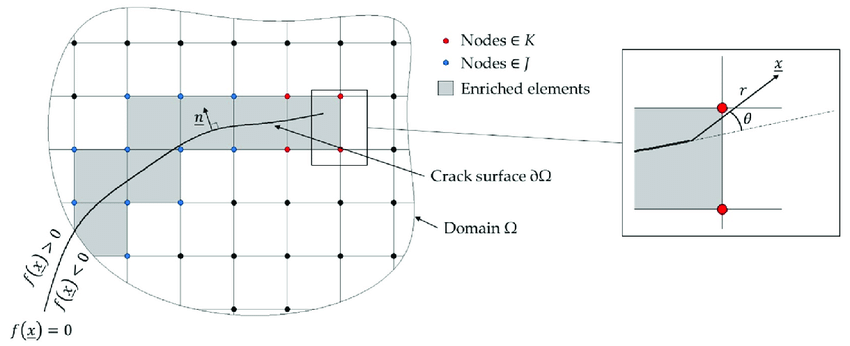
\includegraphics[width=0.7\textwidth]{XFEM.png}
    % \caption{Extended Finite Element Method (XFEM) applied to micro-crack propagation. (a) Crack propagation in a plate with hole, (b) the standard FEM mesh refinement and mesh geometry conformance and (c) the enriched-FEM with uniform mesh enrichments \parencite{swati2019extended}.}
    \caption{Illustration of the extended finite element method (XFEM) approach. The mesh is locally enriched as the crack propagates, in order to avoid remeshing \parencite{de2018delamination}.}
    \label{fig:XFEM}
\end{figure}


In the \textbf{CutFEM} approach \parencite{burman2015cutfem}, the boundary of a given domain is represented on a background grid. CutFEM partitions domains into $\Omega_1$ (exterior) and $\Omega_2$ (interior); separate solution for $\Omega_1$ and $\Omega_2$; captures jumps; integrates over intersections of each element with subdomains; and finally, it weakly imposes boundary and jump conditions (fig. \ref{fig:CutFEM}). 

\begin{figure}[H]
    \centering
    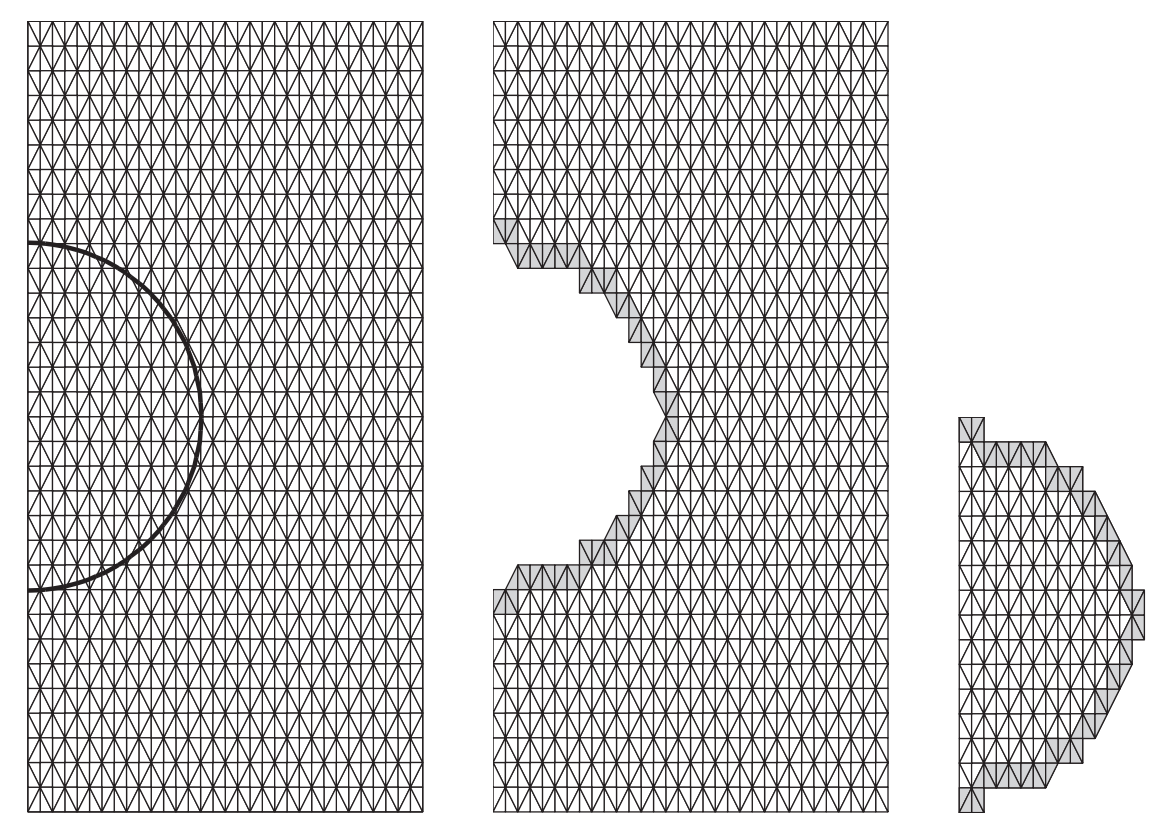
\includegraphics[width=0.6\textwidth]{CutFEM.png}
    \caption{Illustration of the CutFEM approach. A mesh with the interface indicated is being divided into two new meshes. $\Omega_1$ is the exterior (in the middle) and $\Omega_2$ is the interior (on the right). The doubled elements (in both sub-meshes) are shaded \parencite{burman2015cutfem}.}
    \label{fig:CutFEM}
\end{figure}


\textbf{SBM} stands for Shifted Boundary Method \parencite{atallah2020analysis}. In the SBM, the location where boundary conditions are applied is shifted from the true boundary to an approximate (surrogate) boundary; and, at the same time, modified (shifted) boundary conditions
are applied in order to avoid a reduction of the convergence rates of the overall formulation (fig. \ref{fig:SBM}).

\begin{figure}[H]
    \centering
    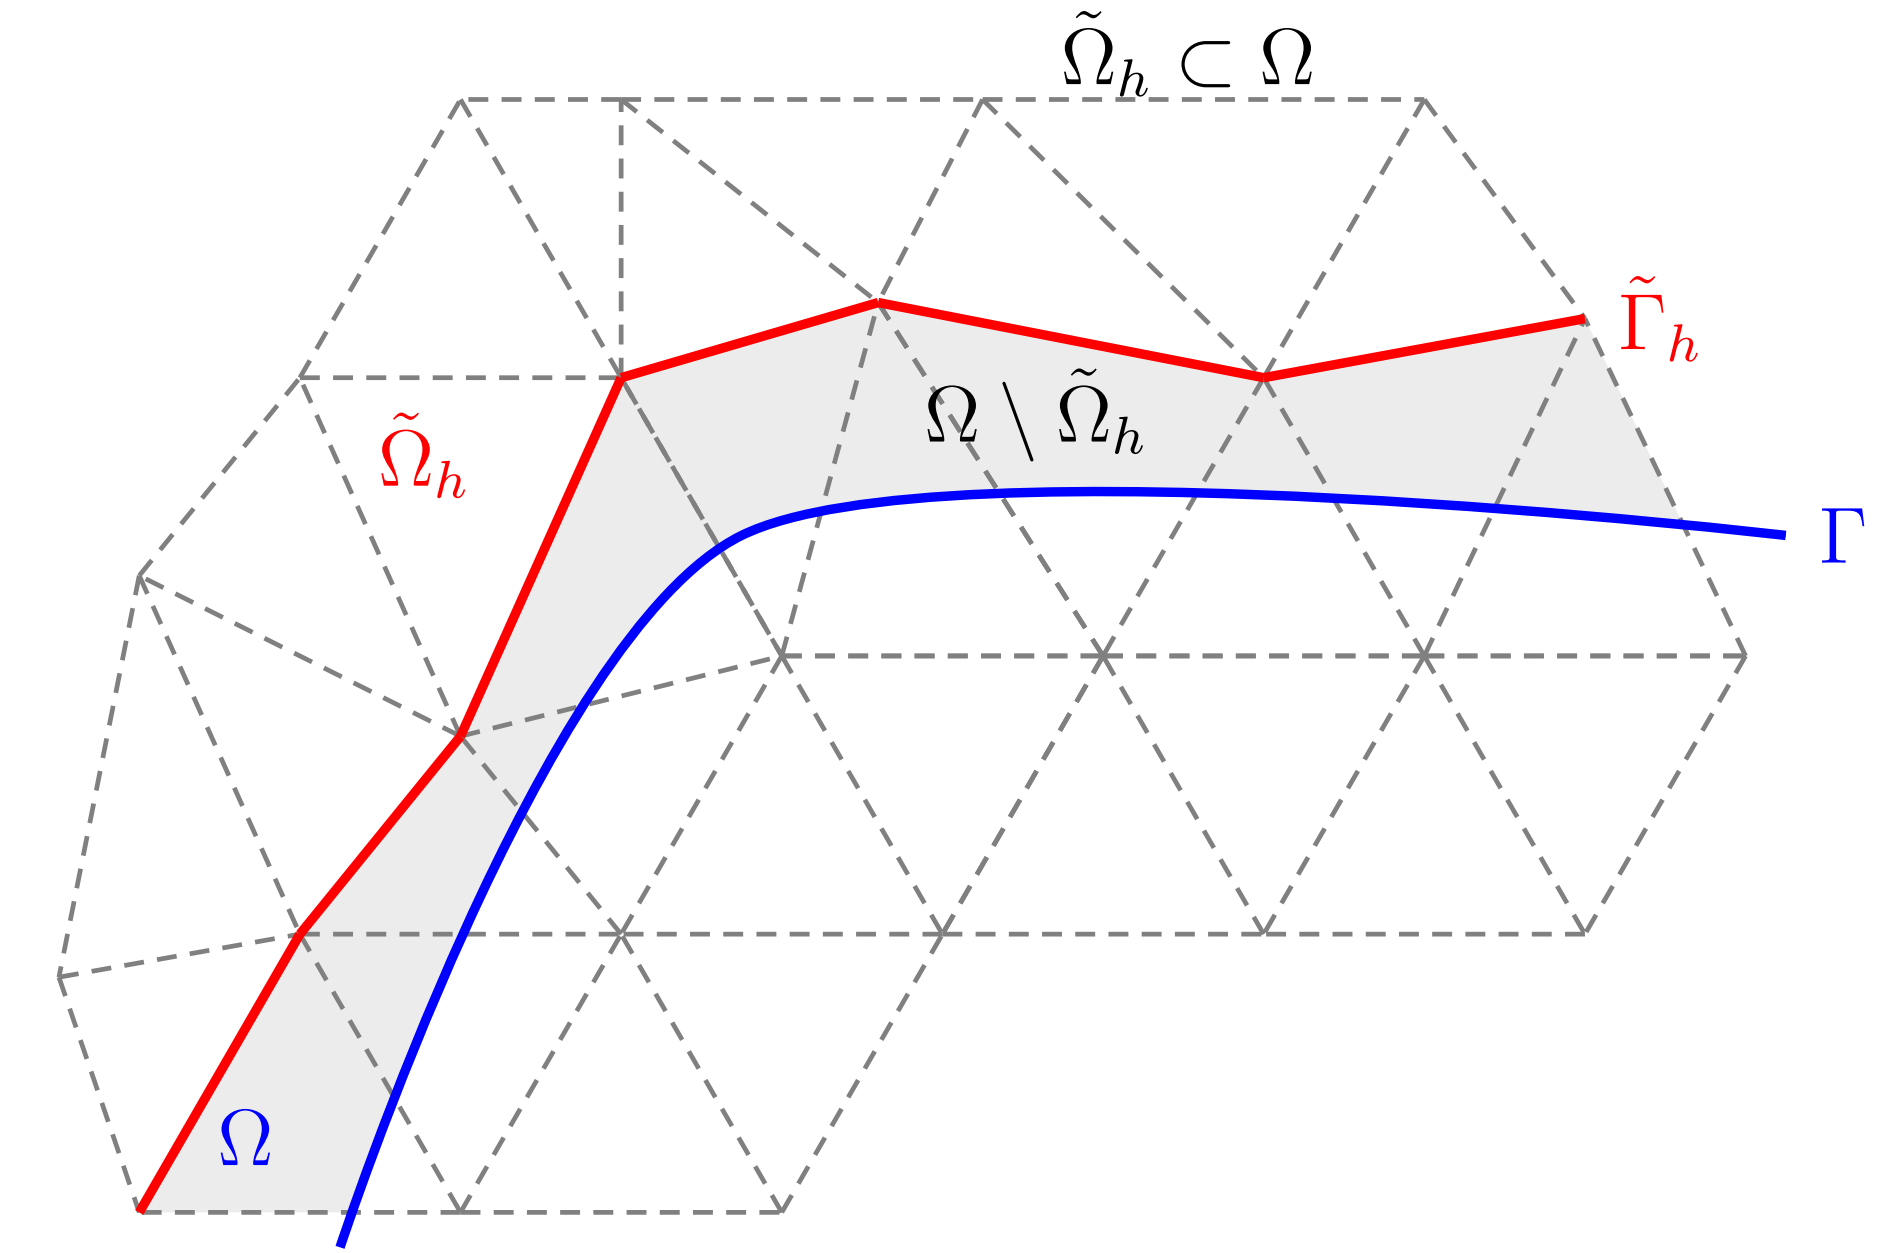
\includegraphics[width=0.5\textwidth]{SBM.png}
    \caption{Illustration of the SBM (Shifted Boundary Method). The original boundary is in blue, while the shifted boundary is in red \parencite{atallah2020analysis}.}
    \label{fig:SBM}
\end{figure}


While these methods (and others based on them) are effective, the integrals over $\Omega$ are kept in the discretization; which in practice, is cumbersome since one needs to implement integrations on the boundary $\Gamma$, and on parts of mesh elements cut by the boundary. Multiple attempts have been made to alleviate this practical difficulty with methods that do not require to perform the
integration on the cut elements, but still need the integration on $\Gamma$. $\phi$-FEM avoids any integration whatsoever on $\Gamma$.


\subsection{Formal presentation of the $\phi$-FEM technique}

As of \today, \phifem has only been developed and tested on the Poisson equation. In the coming paragraphs, we will present the general idea behind the technique, for any common elliptical equation \eqref{eq:problem}. 

In $\phi$-FEM, the boundary condition is carried by the level-set function; and as hinted, all the integrations in $\phi$-FEM are performed on the whole mesh elements, and there are no integrals on $\Gamma$ (even if the mesh element in question is cut by the boundary $\Gamma$). As stated in the introduction, the domain's boundary is the region in space where the level-set function $\phi$ vanishes. This level-set function is chosen such that it remains strictly negative in the interior of the domain. The level-set function is assumed to be smooth, and to behave near $\Gamma$ as the signed distance to $\Gamma$. As an indication, the following problem \footnote{This is eq. \eqref{eq:problem} with a homogeneous Dirichlet boundary condition.}
\begin{align*}
    \exists \, ? \, u \text{ such that }
    \begin{cases}
        \mathcal{L} u = f \quad &\text{ in } \Omega \\ 
        u=0 & \text{ on } \partial \Omega
    \end{cases}
    % \label{eq:classic}
\end{align*}
is reformulated in $\phi$-FEM as (see fig. \ref{fig:ClassicToPhiFEM})
\begin{align*}
    \exists \, ? \, w \text{ such that }
    \begin{cases}
        \mathcal{L} (\phi w) = f \qquad \text{ in } \Omega \\ 
        \text{ where } \Omega = \{ \phi <0 \}, \quad u=\phi w \,.
    \end{cases}
    % \label{eq:phifem}
\end{align*}

\begin{figure}[H]
    \centering
    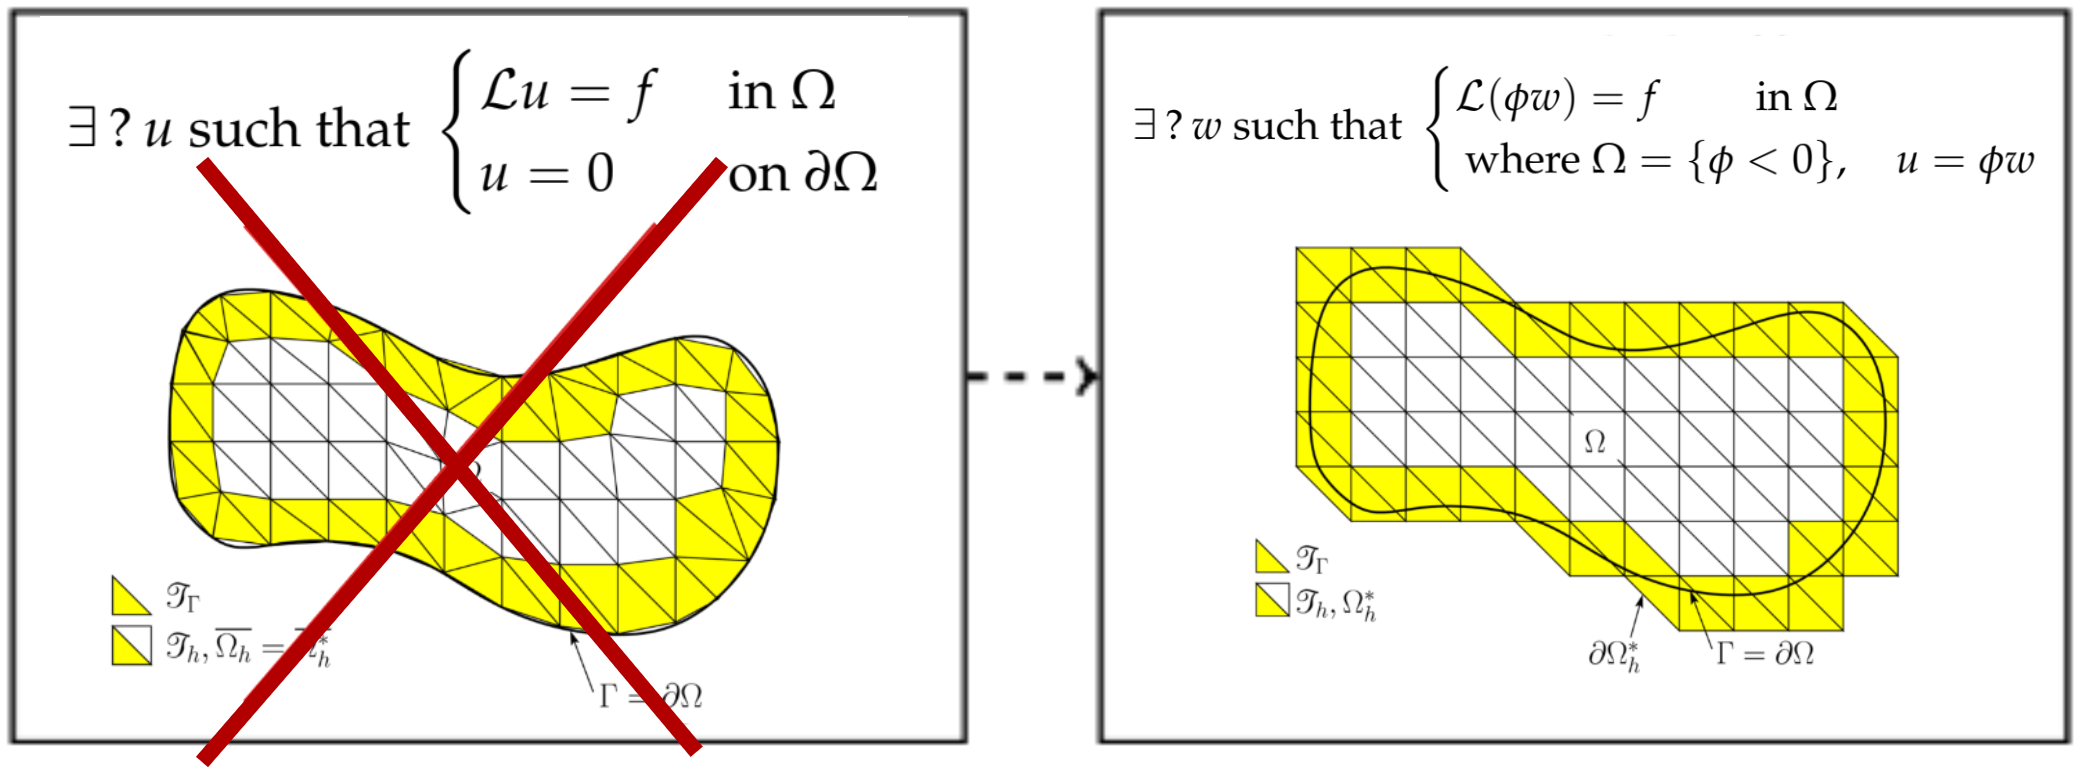
\includegraphics[width=0.7\textwidth]{ClassicToPhiFEM.png}
    \caption{Conversion of a problem from Classic FEM to \phifem in order to avoid complications due to meshing. $\Omega$ and $\partial \Omega$ are defined by the smooth level-set function $\phi$. $\partial\Omega^* = \Gamma^*$ is a fictitious boundary defined by all the cells cut by $\phi$. It is on this boundary that integrations will be performed \parencite{Reference2}.}
    \label{fig:ClassicToPhiFEM}
\end{figure}

As indicated in fig. \ref{fig:ClassicToPhiFEM}, the bounded domain's boundary $\partial\Omega = \Gamma$ is assumed to be smooth and given by a level-set function $\phi$. As stated in the introduction, the domain's boundary will often be the region in space where the level-set function $\phi$ vanishes. This level-set function is chosen such that it remains strictly negative in the interior of the domain:
\begin{align*}
    \Omega := \{ \phi <0 \} \quad \text{and} \quad \Gamma := \{ \phi =0 \}.
\end{align*}
The level-set method allows for treatment of internal boundaries and interfaces without any explicit treatment of the interface geometry. Such a representation is typical in \textbf{immersed boundary techniques}, or \textbf{fictitious domain methods}. It is important for dealing with complex boundaries and problems with evolving surfaces or interfaces. This provides a convenient and an appealing mean for tracking moving interfaces, such as the ones of living organs.

Now let's provide a precise formulation for the Poisson equation \eqref{eq:poisson} using $\phi$-FEM. As $\Omega$ is a bounded domain, we can write $\Omega \subset \mathcal{O} \subset  \mathbb{R}^d$ ($d=2,3$). Let $\Th^{\mathcal{O}}$ be a quasi-uniform simplicial mesh on $\mathcal{O}$ of mesh size $h$. Let's consider, for an integer $l\ge 1$, the finite element space
\begin{eqnarray*}
 V_{h,\mathcal{O}}^{(l)} = \{v_h \in H^1 (\mathcal{O}) : v_h |_T \in \mathbb{P}_l (T)
 \  \forall T \in \mathcal{T}_h^{\mathcal{O}} \} \,,
\end{eqnarray*}
where $\mathbb{P}_l (T)$ stands for the space of polynomials in $d$ variables of degree $\le l$ viewed as functions on $T$. We define $\phi_h$ as 
$$
\phi_h:=I_{h,\mathcal{O}}^{(l)}(\phi) \,,
$$
where $I_{h,\mathcal{O}}^{(l)}$ is the standard Lagrange interpolation operator on $V_{h,\mathcal{O}}^{(l)}$. Henceforth, this function will be used to approximate the physical domain and its boundary. Next we introduce the computational mesh $\mathcal{T}_h$ as the subset of $\Th^{\mathcal{O}}$ composed of the triangles/tetrahedrons having a non-empty intersection with the approximate domain $\{\phi_h<0\}$. We note the domain occupied by $\Th$ as $\Omega_h$ i.e.
$$
\Th:=\{T \in \Th^{\mathcal{O}}:T \cap \{\phi_h<0\} \neq \emptyset\} \quad \text{and} \quad \Omega_h = (\cup_{T \in \Th}T)^o. 
$$
Now the function space will be defined as 
\begin{eqnarray*}
    V_h^{(k)} = \{v_h \in H^1 (\Omega_h) : v_h |_T \in \mathbb{P}_k (T)
    \  \forall ~T \in \mathcal{T}_h \}.
\end{eqnarray*}
The $\phi$-FEM approximation is introduced as follows: 
find $w_h\in V_h^{(k)}$ such that:
\begin{equation}\label{eq:discret prob}
  a_h(w_h,v_h)=l_h(v_h)\mbox{ for all }v_h\in V_h^{(k)},
\end{equation}
where the bilinear form $a_h$ and the linear form $l_h$ are defined by
\begin{equation}
    \label{ahPhiFEM}
   a_h(w,v):=\displaystyle \int_{\Omega_h} \nabla (\phi_h w) \cdot \nabla (\phi_h v) -
\int_{\partial \Omega_h} \frac{\partial}{\partial n} (\phi_h w) \phi_h
   v + G_h (w, v) \,,
\end{equation}	
   and
   \[\displaystyle   l_h(v):= \int_{\Omega_h} f \phi_h v+ G_h^{rhs} (v), \]
with $G_h$ and $G_h^{rhs}$ standing for
\begin{align*} 
 G_h(w, v) &: = \displaystyle\sigma h\sum_{E\in  \mathcal{F}_h^{\Gamma}} 
\int_E \left[ \frac{\partial}{\partial n}
   (\phi_h w) \right] \left[ \frac{\partial}{\partial n} ( \phi_hv)\right]
   + \sigma h^2 \sum_{T \in\Th^{\Gamma}} \int_T \Delta(\phi_h w) \Delta(\phi_h v)  
    \,, \\
   G_h^{rhs} (v) &: =\displaystyle- \sigma h^2\sum_{T \in\Th^{\Gamma}} \int_T f \Delta (\phi_h v)   
   \,,
\end{align*}
where $\sigma> 0$ is an $h$-independent stabilization parameter,  $\Th^{\Gamma}\subset\Th$ contains the mesh elements cut by the approximate boundary $\Gamma_h=\{\phi_h=0\}$, 
\textit{i.e.}
\begin{equation*}
    % \label{eq:def ThGamma}
\Th^{\Gamma}=\{T\in\Th:T\cap\Gamma_h\neq\emptyset\},
\quad
\Omega_h^{\Gamma}:=\left(\cup_{T\in \mathcal{T}_h^{\Gamma}}T\right)^o ;
\end{equation*}
and $\mathcal{F}_h^{\Gamma}$ collects the interior facets of the mesh $\Th$ either cut by $\Gamma_h$ or belonging to a cut mesh element
\begin{equation*}
  \mathcal{F}_h^{\Gamma} = \{E \text{ (an internal facet of } \mathcal{T}_h)
  \text{ such that } \exists T \in \mathcal{T}_h : T \cap \Gamma_h \neq
  \emptyset \text{ and } E \in \partial T\}.
%  \{E \text{ (an internal edge of } \mathcal{T}_h)
%  \text{ such that } \exists T \in \mathcal{T}_h : T \cap \Gamma_h \neq
%  \emptyset \text{ and } E \in \partial T\}.
\end{equation*}
The brackets inside the integral over $E\in\mathcal{F}_h^{\Gamma}$ in the formula for $G_h$ stand for the jump over the facet $E$. The first part in $G_h$ actually coincides with the ghost penalty as introduced in \parencite{burman2010ghost} for $P_1$ finite elements. 


\section{The Poisson problem}

\subsection{Using classic FEM}
% The weak formulation is obtained by replacing $\sigma$ in \eqref{eq:classic} with the gradient function, multiplying both sides by $v$, and applying Green's formula. In the FEM approximation space $V_h$, the goal is to find $u_h$ such that $a(u_h,v)=l(v) \, \, \forall v \in V_h$, with $a_h$ a bilinear form, and $l_h$ a lieanr such that
% \begin{align}
%     \notag
%     a(u,v) &=\int_{\Omega_h} \nabla u \cdot \nabla v \\
%     l(v) &= \int_{\Omega_h} fv
% \end{align}

The basis for the weak formulation has been laid down in \eqref{eq:PoissonClassic}. The values for $f$, and the domain $\Omega$ need to be defined in order to run the test cases. Moreover, the exact solution $u$ has to be known in order to perform a convergence study. 

The classic FEM technique has been tested on a particular case. The case in question is the \textbf{test case 1} from \cite[p.15]{Reference3}. The corresponding parameters are presented below \footnote{Notice that $f$ is very cumbersome to compute manually ; that is why we will be using Sympy for such tasks.}, and the result is shown in fig. \ref{fig:ClassicPoisson2}.
\begin{align}
    \begin{cases}
    \Omega = \left\{ (x,y)\in\mathbb{R}^2: \left( x-\frac{1}{2} \right)^2 + \left( y-\frac{1}{2} \right)^2 < \frac{1}{8}  \right\} \\
    u(x,y)= -\left( \frac{1}{8} - \left( x-\frac{1}{2} \right)^2 - \left( y-\frac{1}{2} \right)^2 \right) \exp(x) \sin(2\pi y)\\
    f(x,y) = -\frac{\partial^2 u}{\partial x^2}(x,y) -\frac{\partial^2 u}{\partial y^2}(x,y)
    \end{cases}
    \label{eq:test2}
\end{align}

% \begin{itemize}
%     \item The first case's paremeters are presented below, and the result in fig. \ref{fig:ClassicPoisson}.
%     \begin{align}
%         \begin{cases}
%         \Omega =  \left\{ (x,y)\in\mathbb{R}^2: x^2 + y^2 < 1  \right\} \\
%         u(x,y)=\frac{(1-x^2-y^2)}{4}\exp(x) \times \sin(y) \\
%         f(x,y) = \exp(x) (x \cos(x) + (1+y)\sin(y))
%         \end{cases}
%         \label{eq:test1}
%     \end{align}
    
    % The first (fig. \ref{fig:ClassicPoisson}) has been obtained on a unit disk with $f(x,y) = \exp(x) (x*\cos(x) + (1+y)*\sin(y))$. The exact solution, needed for the convergence study, is $u(x,y)=\frac{(1-x^2-y^2)}{4}\exp(x) * \sin(y)$.

    %\item The case in question is the \textit{test case 1} from \parencite[p.15]{Reference3}. The corresponding parameters are presented below \footnote{Notice that $f$ is very cumbersome to compute. The $Sympy$ library will help with that.}, and the result in fig. \ref{fig:ClassicPoisson2}.
    % \begin{align}
    %     \begin{cases}
    %     \Omega = \left\{ (x,y)\in\mathbb{R}^2: \left( x-\frac{1}{2} \right)^2 + \left( y-\frac{1}{2} \right)^2 < \frac{1}{8}  \right\} \\
    %     u(x,y)= \left( \frac{1}{8} - \left( x-\frac{1}{2} \right)^2 - \left( y-\frac{1}{2} \right)^2 \right) \exp(x) \sin(2\pi y)\\
    %     f(x,y) = -\frac{\partial^2 u}{\partial x^2}(x,y) -\frac{\partial^2 u}{\partial y^2}(x,y)
    %     \end{cases}
    %     \label{eq:test2}
    % \end{align}
    
% \end{itemize}

% \begin{figure}[H]
%     \centering
%     \begin{subfigure}[b]{0.45\textwidth}
%         % \centering
%         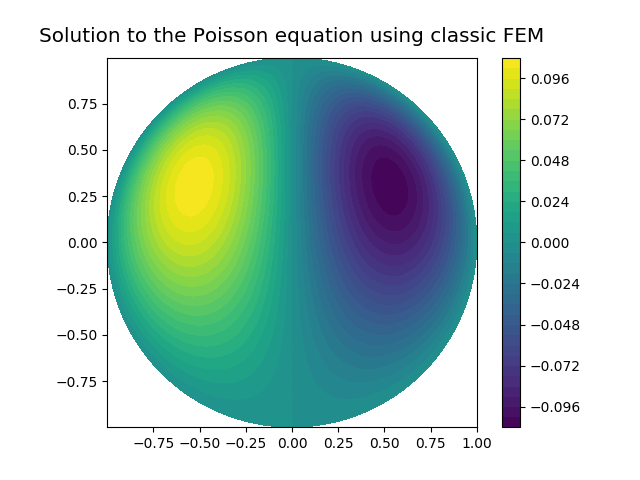
\includegraphics[width=\textwidth]{ClassicSol.png}
%         \caption{Solution}
%         \label{fig:ClassicSol}
%     \end{subfigure}
%     % \hfill
%     \begin{subfigure}[b]{0.45\textwidth}
%         % \centering
%         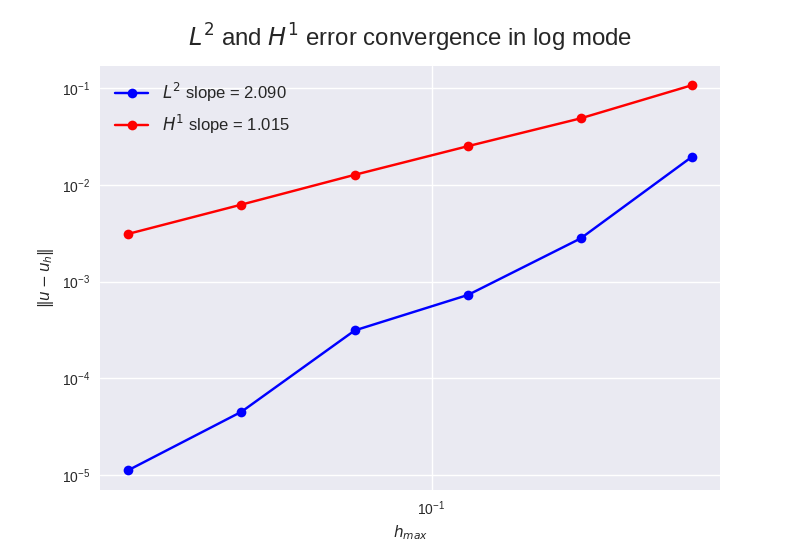
\includegraphics[width=\textwidth]{ClassicCvgStudy.png}
%         \caption{Convergence study}
%         \label{fig:ClassicCvgStudy}
%     \end{subfigure}
%     % \hfill
%        \caption{Results obtained when applying the classic FEM tecnhique to the Poisson equation on first case (\eqref{eq:test1})}
%        \label{fig:ClassicPoisson}
% \end{figure}

\begin{figure}[H]
    \centering
    \begin{subfigure}[b]{0.45\textwidth}
        % \centering
        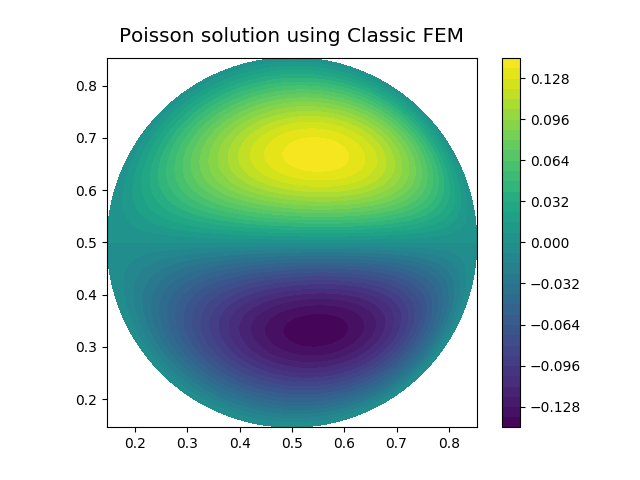
\includegraphics[width=\textwidth]{ClassicSol2.png}
        \caption{Solution}
        \label{fig:ClassicSol2}
    \end{subfigure}
    % \hfill
    \begin{subfigure}[b]{0.45\textwidth}
        % \centering
        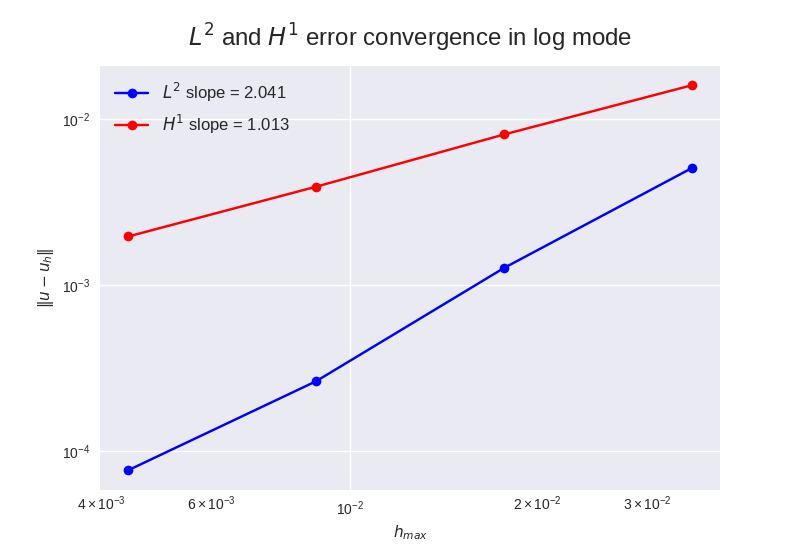
\includegraphics[width=\textwidth]{ClassicCvgStudy2.png}
        \caption{Convergence study}
        \label{fig:ClassicCvgStudy2}
    \end{subfigure}
    % \hfill
       \caption{Results obtained when applying the classic FEM technique to the Poisson equation \eqref{eq:test1redef}. The $H^1$ norm presented in (B) is the norm $\Vert u - u_h\Vert_{1, \Omega}$. These results confirm what we expect since and will serve as a reference for the following results. The red and blue plots in (B) indicate the relative error.}
       \label{fig:ClassicPoisson2}
\end{figure}
The results we obtained (fig. \ref{fig:ClassicCvgStudy2}) fully match the expected theoretical framework. For the Poisson problem, the expected convergence is described below \parencite[p.121]{ern2013theory}. As $u \in H^1(\Omega)$\footnote{We can also prove that $u \in H^2(\Omega)$ using the elliptic regularity theorem.}, we know that the error converges according to the inequalities \footnote{$u$ is the exact solution interpolated in the variational space, and $u_h$ is our FEM approximation.}:
\begin{align}
    \Vert u - u_h \Vert_{L^2(\Omega)} \leq C h^2 \vert u \vert_{H^2(\Omega)} \,, \\
    \Vert u - u_h \Vert_{H^1(\Omega)} \leq C h^1 \vert u \vert_{H^2(\Omega)} \,.
\end{align} 



\subsection{Using $\phi$-FEM}
% Just as in classic FEM, the weak formulation is obtained by replacing $\sigma$ in \eqref{eq:phifem} by the gradient. The same steps lead to finding $w_h$ such that $a(w_h,v)=l(v) \, \, \forall v \in V_h$, and the solution $u_h= \phi w_h$. In this case, $a$ and $l$ are defined as in \eqref{eq:poisson}. 

The basis for the Poisson problem in $\phi$-FEM have been laid in \eqref{ahPhiFEM}. Multiple parameters must be defined in order to have a proper test case.

% Repeating the same order as the cases in classic FEM, we see that:
% \begin{itemize}
%     \item The first case defined in classic FEM as \eqref{eq:test1} can be redefined in $\phi$-FEM as follows . The result is presented at (\textit{NOT YET BEEN IMPLEMENTED})
%     \begin{align}
%         \begin{cases}
%         \mathcal{O} = \ldots \\
%         \phi(x,y) = \frac{1 - x^2 - y^2}{4} \\
%         u(x,y)=\phi(x,y) \times \exp(x) \times \sin(y) \\
%         f(x,y) = \exp(x) (x \cos(x) + (1+y) \sin(y))
%         \end{cases}
%         \label{eq:test1redef}
%     \end{align}
    
%     \item The second test case defined in classic FEM as \eqref{eq:test2} is redefined below. The result is presented at fig. \ref{fig:StabPoisson}
%     \begin{align}
%         \begin{cases}
%         \mathcal{O} = [0,1]\times[0,1] \\
%         \phi(x,y) = -\frac{1}{8} + \left( x-\frac{1}{2} \right)^2 + \left( y-\frac{1}{2} \right)^2 \\
%         u(x,y)=\phi(x,y) \times \exp(x) \times \sin(2\pi y) \\
%         f(x,y) = -\frac{\partial^2 u}{\partial x^2}(x,y) -\frac{\partial^2 u}{\partial y^2}(x,y) \\
%         \sigma = 20
%         \end{cases}
%         \label{eq:test1redef}
%     \end{align}
% \end{itemize}

Let's repeat the same test case we did in classic FEM. The test case, defined in classic FEM as \eqref{eq:test2}, is redefined below. The result is presented at fig. \ref{fig:StabPoisson}.
\begin{align}
    \begin{cases}
    \mathcal{O} = [0,1]\times[0,1] \\
    \phi(x,y) = -\frac{1}{8} + \left( x-\frac{1}{2} \right)^2 + \left( y-\frac{1}{2} \right)^2 \\
    u(x,y)=\phi(x,y) \times \exp(x) \times \sin(2\pi y) \\
    f(x,y) = -\frac{\partial^2 u}{\partial x^2}(x,y) -\frac{\partial^2 u}{\partial y^2}(x,y) \\
    \sigma = 20
    \end{cases}
    \label{eq:test1redef}
\end{align}

\begin{figure}[H]
    \centering
    \begin{subfigure}[b]{0.45\textwidth}
        % \centering
        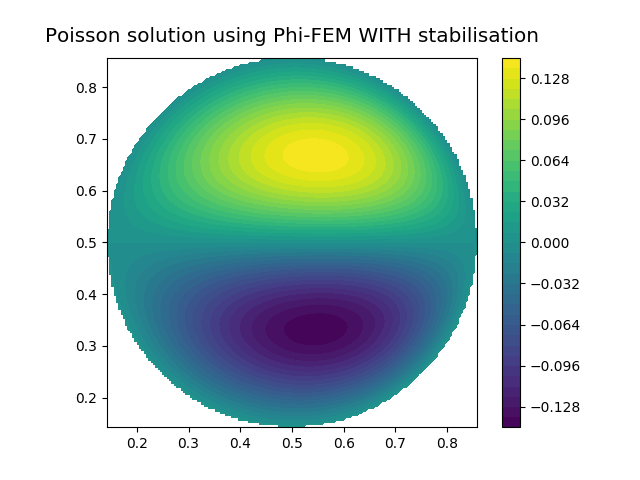
\includegraphics[width=\textwidth]{StabSol.png}
        \caption{Solution}
        \label{fig:StabSol}
    \end{subfigure}
    % \hfill
    \begin{subfigure}[b]{0.45\textwidth}
        % \centering
        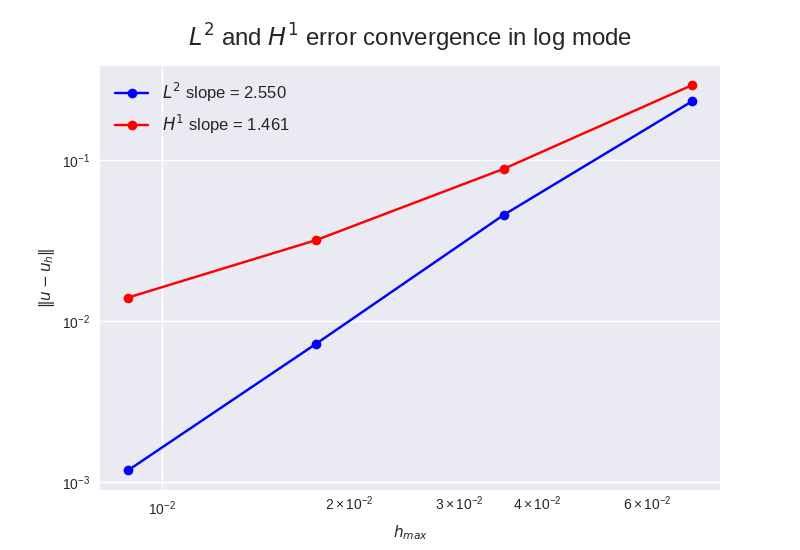
\includegraphics[width=\textwidth]{StabCvgStudy.png}
        \caption{Convergence study}
        \label{fig:StabCvgStudy}
    \end{subfigure}
    % \hfill
       \caption{Results obtained when applying the $\phi$-FEM technique with stabilization to the Poisson equation. The $H^1$ norm presented in (B) is the norm $\Vert u - u_h\Vert_{1, \Omega\cap\Omega_h}$, for better comparison with the classic FEM case. These results confirm what we expected, with better slopes compared to fig. \ref{fig:ClassicPoisson2}.}
       \label{fig:StabPoisson}
\end{figure}
These results were expected. In fact, they are better than expected, and much better than classic FEM. When the right-hand side of the Poisson equation $f$ belongs to $H^k(\Omega_h\cup\Omega)$, the convergence rates should be \parencite[p.4]{Reference3}\footnote{A number of assumptions had to be made. Those are not repeated here.}:  
\begin{align}
    | u - u_h|_{1, \Omega\cap\Omega_h} \le Ch^k \|f \|_{k, \Omega\cup\Omega_h}  \,,\\
    \| u - u_h\|_{0, \Omega} \le Ch^{k+1/2} \|f \|_{k, \Omega_h} \,.
\end{align}	

Concerning the fact that the solution (on the domain's boundary) in fig. \ref{fig:StabSol} doesn't look as smooth as in fig. \ref{fig:ClassicSol2}, we can say that it was perfectly anticipated due to the way the meshes are generated in FEniCS. The reason is that: using triangles, a 2D disk is very easily meshable, which is what is done in Classic FEM; thus the smoothness on the boundary. The \phifem  approach will come in handy when the geometry will not be meshable, and will thus have to be immersed in a larger mesh.

\section{The elasticity equation}


\subsection{Using Classic FEM}

\begin{figure}[H]
    \centering
    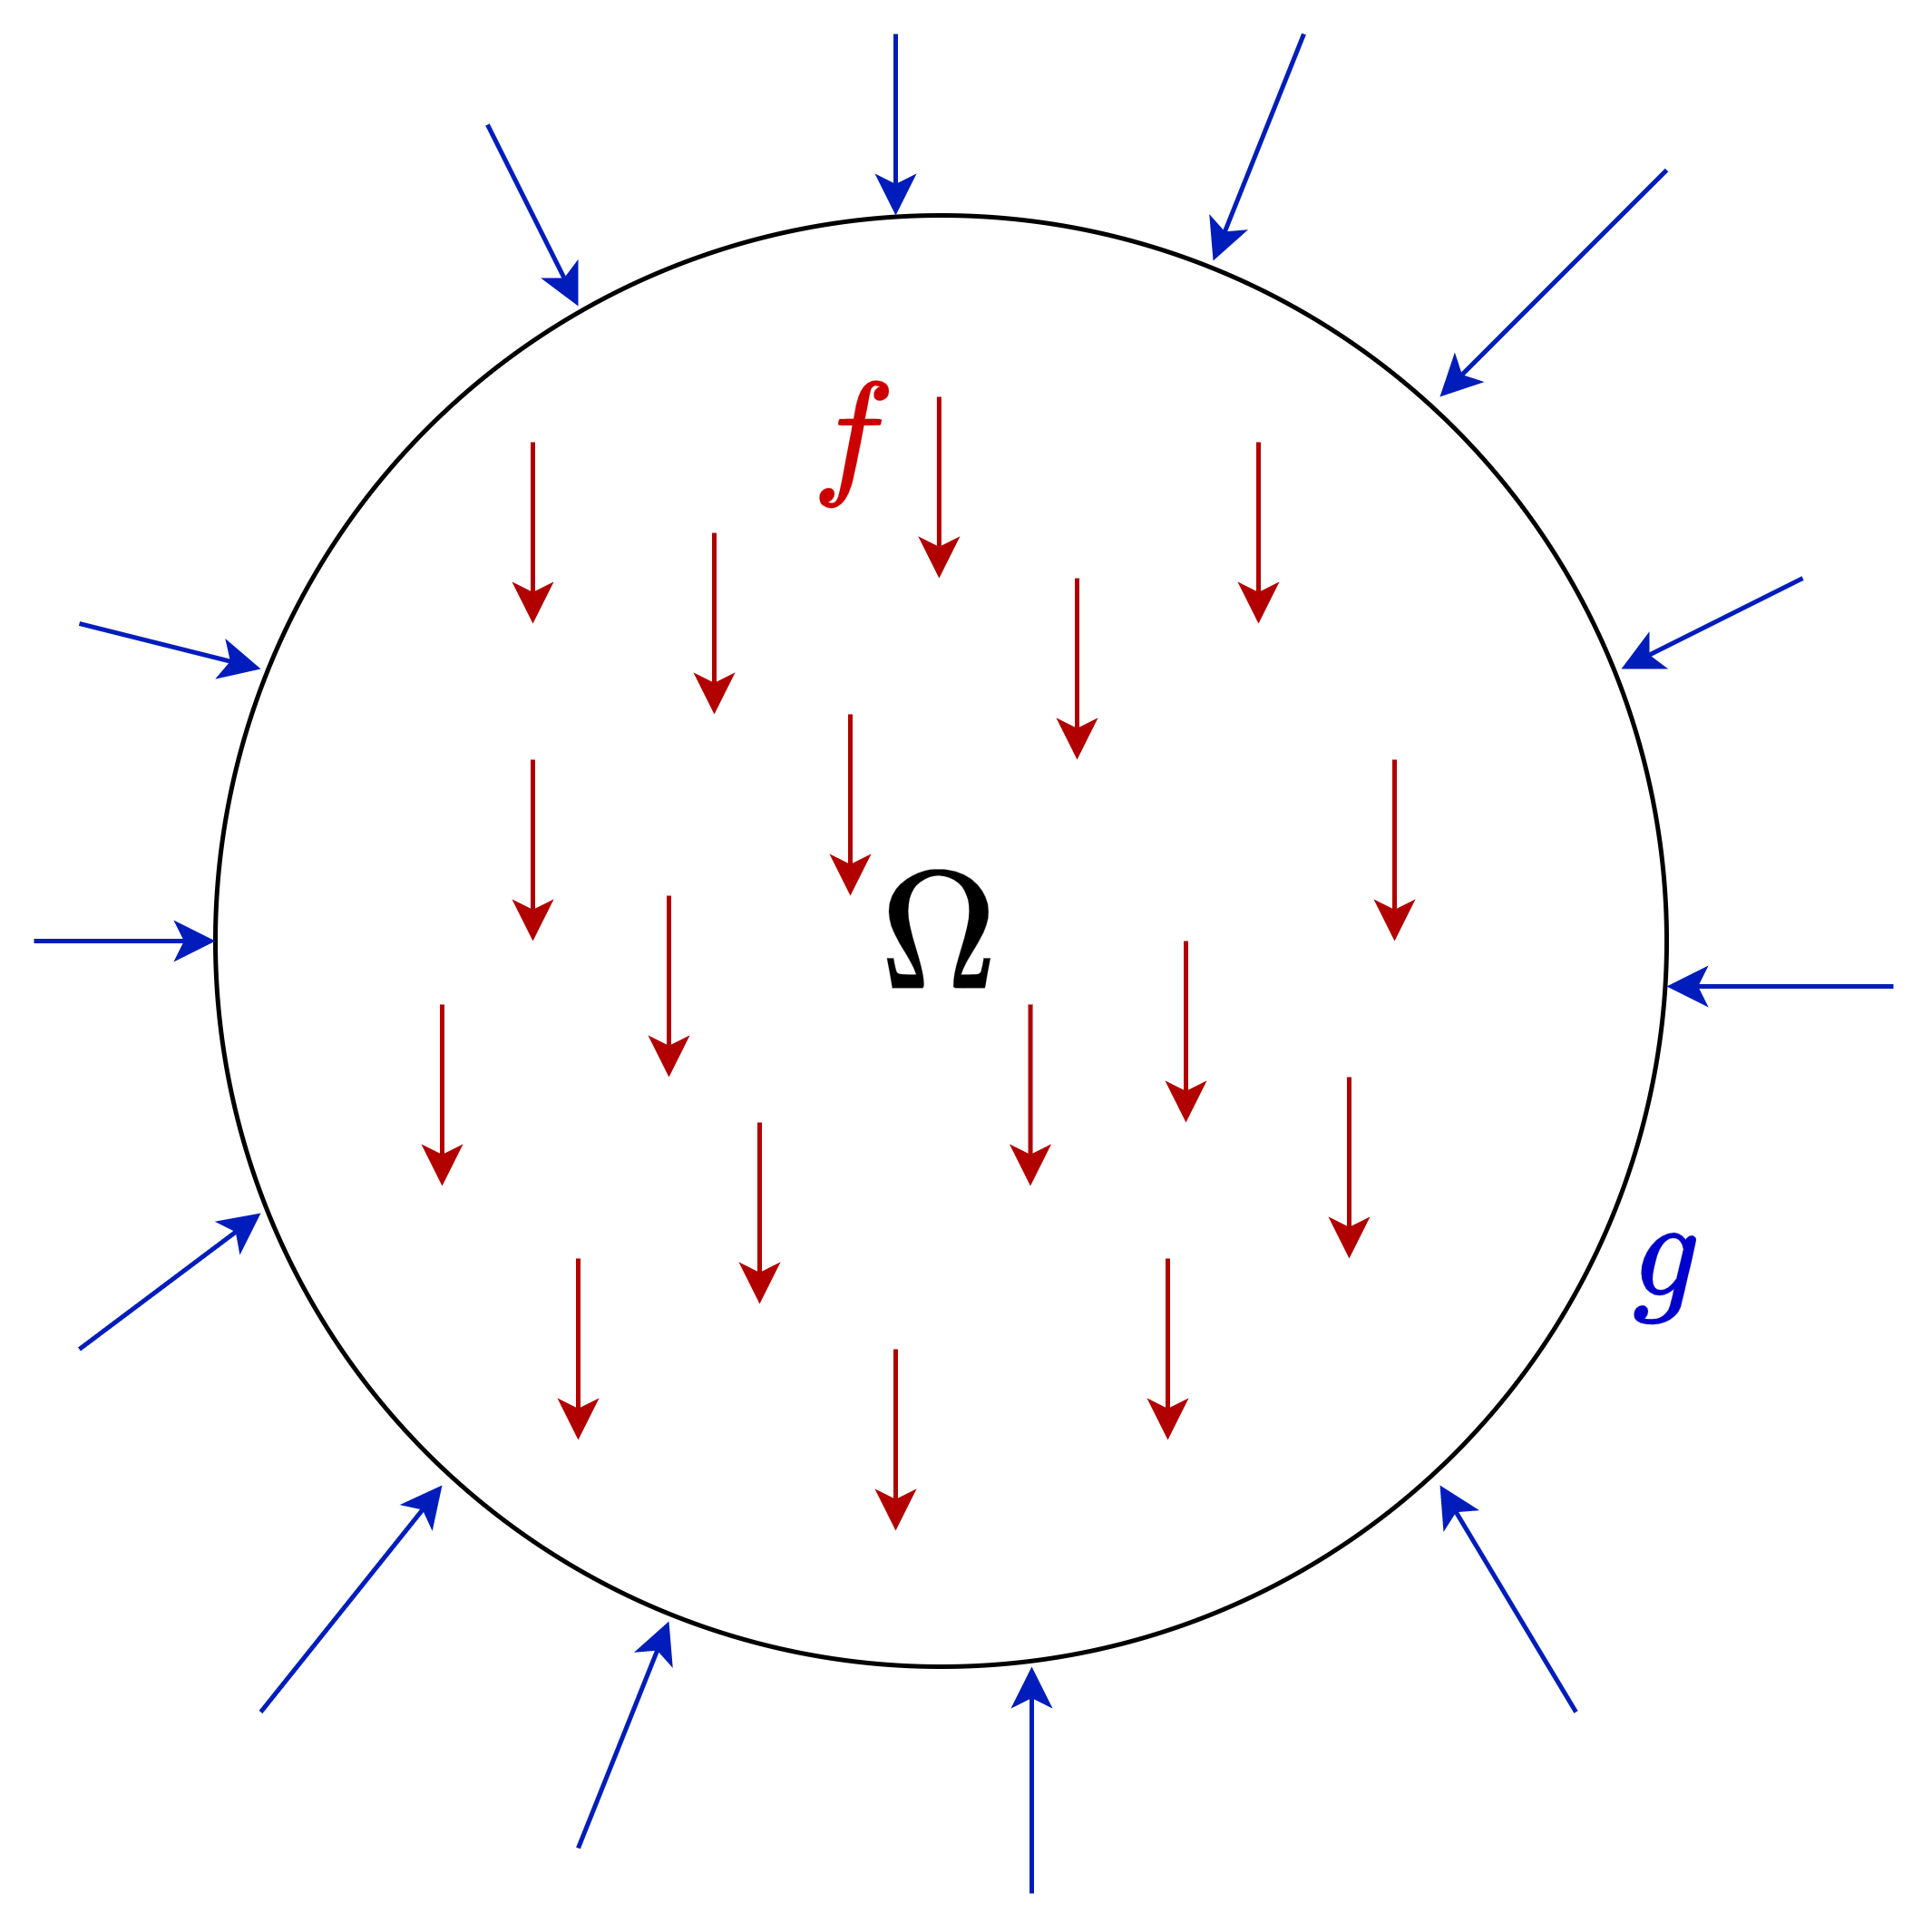
\includegraphics[width=0.3\textwidth]{Clamped.png}
    % \caption{Illustration of the linear elasticity (small deformations) problem. The boundary $ \partial \Omega_D$ is clamped, whereas a normal load $g: \partial \Omega_N \mapsto \mathbb{R}^3$ is imposed on $\partial\Omega_N$. $f$ is the external force applied to the beam's particles i.e the gravity. $f$ and $g$ are assumed smooth enough \parencite[p.153]{ern2013theory}.}
    \caption{Illustration of a linear elasticity problem (with small deformations). The domain $ \Omega$ is a disk. The vertical force $f$ can be associated to the gravity. The displacement vector $g$ on the boundary is fixed.}
    \label{fig:beam}
\end{figure}


With $u: \Omega \mapsto \mathbb{R}^d$, $\sigma(u)$ and $\varepsilon (u) = \frac{1}{2}(\nabla u + \nabla u^T)$ representing (respectively) the displacement, the stress and the strain tensors, the model problem (illustrated at fig. \ref{fig:beam}) is as follows \parencite[p.153]{ern2013theory} :
\begin{align}
    \begin{cases}
    \nabla \cdot \sigma(u) + f = 0 &\quad \text{in } \Omega \,\\   
    \sigma(u) = \lambda \, \text{tr}(\varepsilon(u)) \mathcal{I} + 2 \mu \varepsilon(u)  &\quad \text{in } \Omega \,\\
    u = g &\quad \text{on } \partial\Omega \,
    \end{cases}
    \label{eq:elasticity}
\end{align}
where $\lambda$ and $\mu$ are the Lamé coefficients. With $d=2,3$, the test functions are taken in the functional space 
$$
V = \left[  H_0^1(\Omega)\right]^d \,.
$$
We have
\begin{align*}
    - \int_{\Omega} \nabla \cdot \sigma(u) \cdot v &= \int_{\Omega} f \cdot v \qquad \forall v \in V
\end{align*}
equivalent to (using Green's formula)
\begin{align*}
    \int_{\Omega} \sigma(u) : \nabla v - \int_{\partial\Omega} (\sigma(u) \cdot n) \cdot v &= \int_{\Omega} f \cdot v \,. \qquad \tag{$\star$}
\end{align*}
Lets remember that the matrix dot product (double dots ":" operation) of a symmetric and a skew-symmetric matrix is zero. We know that $\sigma(u)$ is symmetric according to its definition in \eqref{eq:elasticity}. We then decompose $\nabla v$ into the sum of a symmetric part $\nabla^s v  = \frac{1}{2}\left( \nabla v + \nabla v^T  \right)$ and a skew-symmetric part $\nabla^a v  = \frac{1}{2}\left( \nabla v - \nabla v^T  \right)$. Since $\sigma(u):\nabla^a v = 0$, we get (by also taking $u = 0$ on the boundary) :  
\begin{align*}
    \int_{\Omega} \sigma(u) : \nabla^s v = \int_{\Omega} f \cdot v  \,, 
\end{align*}
that is
\begin{align*}
    \int_{\Omega} \sigma(u) : \varepsilon(v) = \int_{\Omega} f \cdot v  \,.
\end{align*}
This leads to the following weak formulation in classic FEM
\begin{align}
    \text{Seek } u \in G+V \text{ such that} \quad a(u,v)=l(v), \quad \forall v \in V \,,
\end{align}
where $G$ as is a set of functions such that its elements' "trace" on the boundary $\partial\Omega$ is equal to $g$. The functionals $a$ and $l$ are defined as 
$$
a(u,v) = \int_{\Omega} \sigma (u) : \varepsilon (v) \,
$$
and
$$
l(v) = \int_{\Omega} f\cdot v \,.
$$

Let's look at the a priori error estimation \parencite[p.159]{ern2013theory}. As $u \in V = \left[  H^1(\Omega)\right]^d$\footnote{It is important to note that $u \in \left[  H^2(\Omega)\right]^d$ according to the elliptic regularity theorem.}, we know that the errors converge according to the inequalities below\footnote{As with the Poisson problem, $u$ is the exact solution interpolated in the variational space, and $u_h$ is our finite element approximation.}:
\begin{align}
    \Vert u - u_h \Vert_{L^2(\Omega)^d} \leq C h^2 \vert u \vert_{H^2(\Omega)^d} \\
    \Vert u - u_h \Vert_{H^1(\Omega)^d} \leq C h^1 \vert u \vert_{H^2(\Omega)^d}
\end{align} 

The classic FEM technique has been tested in FEniCS for the elasticity equation on a particular case\footnote{Let's note that $f(x,y)$ was computed using the Sympy library ; the result is too long to the printed here.}. The results, implemented in FEniCS in a 2D variational space, are presented in fig. \ref{fig:ClassicElas}.
\begin{align}
    \begin{cases}
    \Omega = \left\{ (x,y)\in\mathbb{R}^2: \left( x-\frac{1}{2} \right)^2 + \left( y-\frac{1}{2} \right)^2 < \frac{1}{8}  \right\} \\
    u(x,y)= \begin{pmatrix}
        2x + \sin(x)\exp(y) \\ \frac{x}{2} + \cos(x) - 1
    \end{pmatrix}  \\
    f(x,y) = -\nabla \cdot \sigma(u(x,y)) \\
    g(x,y) = u(x,y)
    \end{cases}
    \label{eq:test3}
\end{align}

\begin{figure}[H]
    \centering
    \begin{subfigure}[b]{0.40\textwidth}
        % \centering
        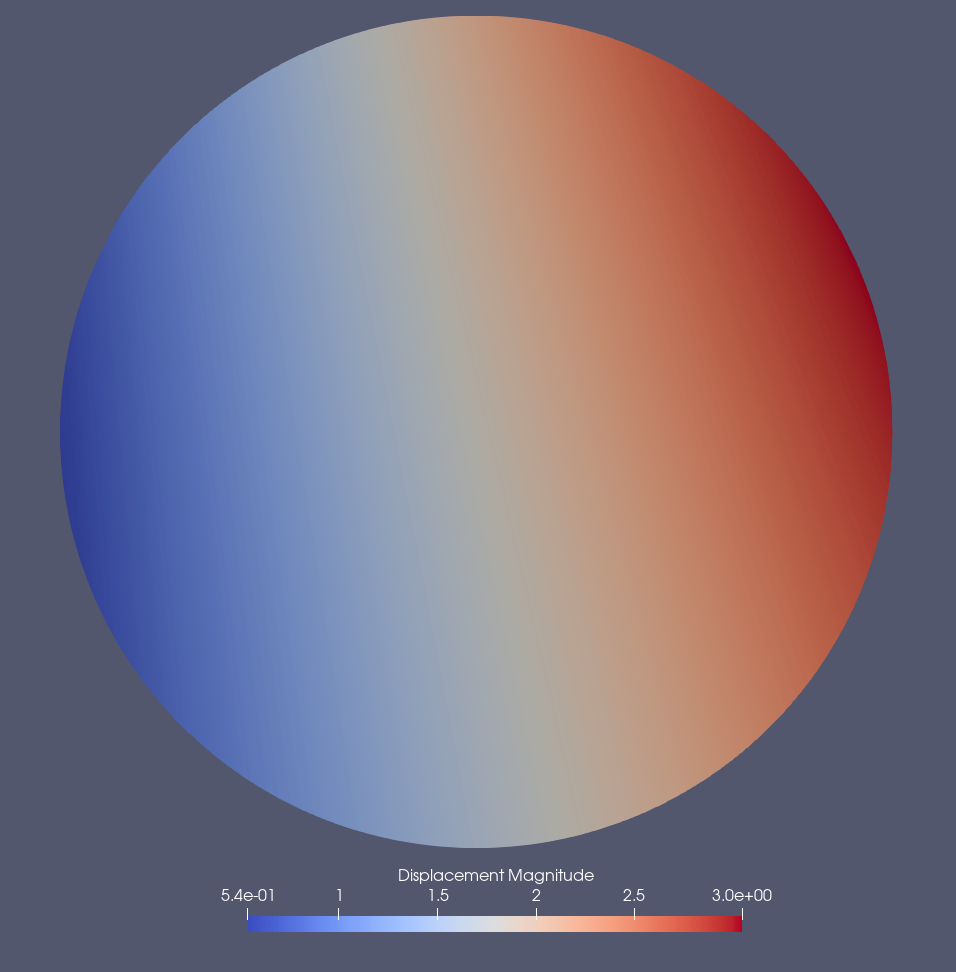
\includegraphics[width=\textwidth]{ClassicElasPara1.png}
        \caption{Solution's magnitude in Paraview}
        \label{fig:Para1}
    \end{subfigure}
    % \hfill
    \begin{subfigure}[b]{0.50\textwidth}
        % \centering
        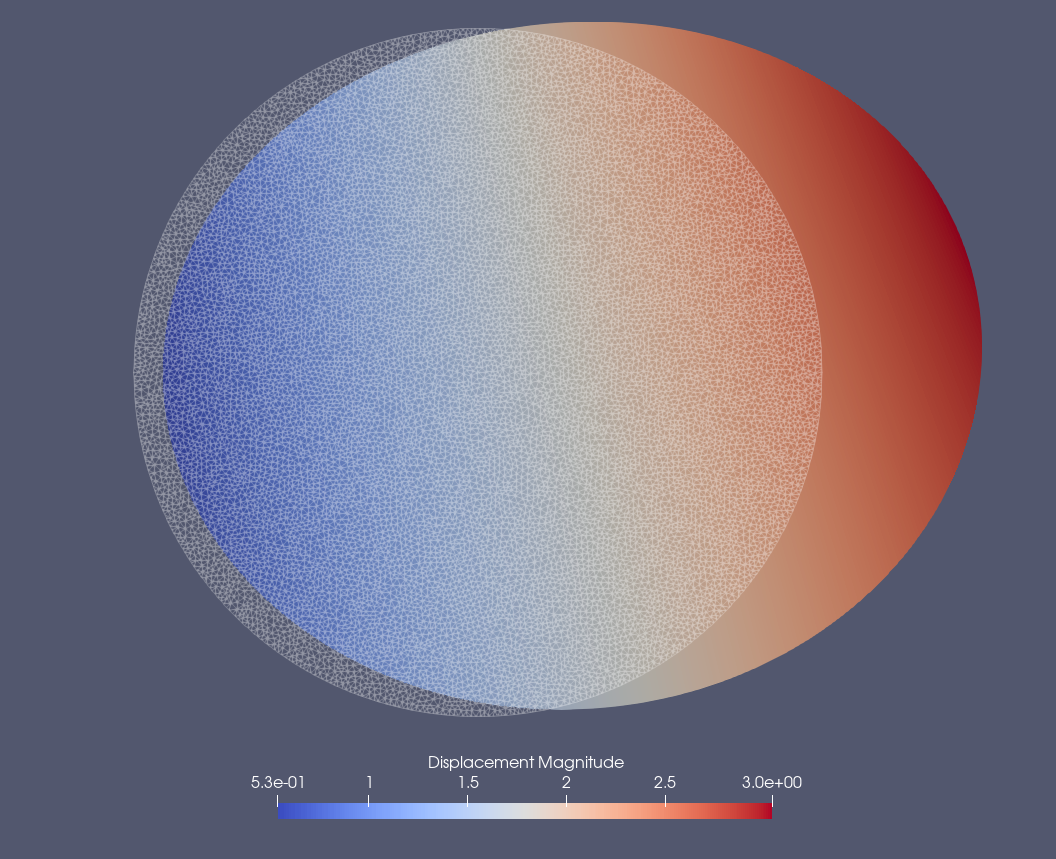
\includegraphics[width=\textwidth]{ClassicElasPara2.png}
        \caption{Solution warped by vector in Paraview}
        \label{fig:Para2}
    \end{subfigure}
    \begin{subfigure}[b]{0.45\textwidth}
        % \centering
        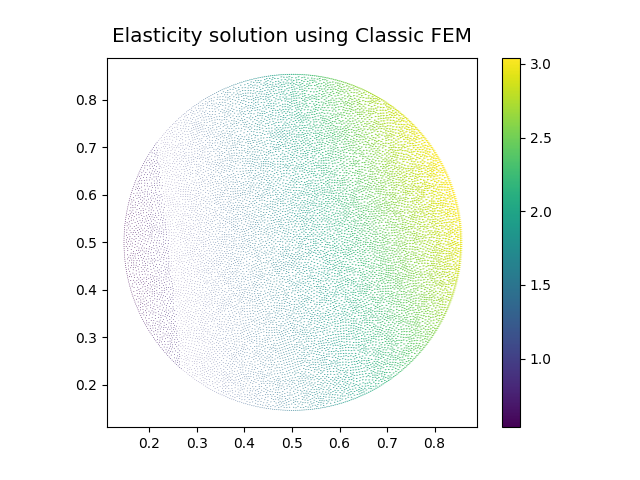
\includegraphics[width=\textwidth]{ClassicElasSol.png}
        \caption{Solution's components (vector) in Matplotlib}
        \label{fig:ClassicElasSol}
    \end{subfigure}
    % \hfill
    \begin{subfigure}[b]{0.45\textwidth}
        % \centering
        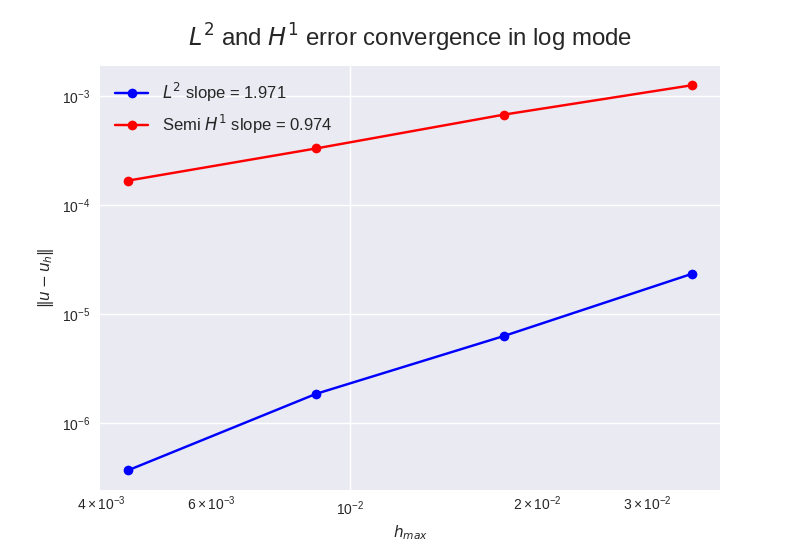
\includegraphics[width=\textwidth]{ClassicElasCvg.png}
        \caption{Convergence study}
        \label{fig:ClassicElasCvg}
    \end{subfigure}
    % \hfill
       \caption{Results obtained when applying the classic FEM technique to the elasticity equation \eqref{eq:elasticity}. The warp by vector (B) shows that the elastic material is expanding to its right, but contracting to its left. The convergence study (D) in done with relative errors. The $H^1$ slope indicated in (D) is the $H^1$ semi-norm $\vert u - u_h\vert_{1, \Omega}$.}
       \label{fig:ClassicElas}
\end{figure}


\subsection{Using \phifem}

Let's derive the weak formulation based on \eqref{eq:elasticity}\footnote{Note that we won't include the subscript $h$ as we did for the Poisson problem's \phifem formulation; because what we are giving next is just a general framework for the technique, not its FEM approximation. By doing so, our notations are simpler, and without ambiguity.}. Since our whole boundary will consist of Dirichlet conditions, we go from eq. ($\star$) to write $u=\phi w + g$, and $v$ becomes $\phi v$\footnote{We turn $v$ into $\phi v$ for ease of use. As $v$ is just a test function, we could have written $v = \phi v'$ instead, and continued with $v'$.}. We use Green's formula just as in the classic FEM, and we get
\begin{align*}
    \int_{\Omega} \sigma(\phi w + g) : \varepsilon(\phi v) - \int_{\partial\Omega} (\sigma(\phi w + g) \cdot n)  \cdot \phi v = \int_{\Omega} f \cdot \phi v \,.
\end{align*}
This gives us the "early" form of the weak formulation
\begin{align}
    \int_{\Omega} \sigma(\phi w) : \varepsilon(\phi v) - \int_{\partial\Omega} (\sigma(\phi w) \cdot n) \cdot \phi v = \int_{\Omega} f \cdot \phi v - \int_{\Omega} \sigma(g) : \varepsilon(\phi v) + \int_{\partial\Omega} (\sigma(g) \cdot n) \cdot \phi  v \,.
    \label{eq:1}
\end{align}
Now let's consider the ghost cells $\mathcal{T}_h^{\Gamma}$ \footnote{These are the macro mesh's cells that are cut by the level-set function $\phi$, and those that have at least one edge in common with a cut cell.} and their edges $\mathcal{F}_h^{\Gamma}$, and apply stabilization terms\footnote{These terms will later be penalized by a constant $\sigma_{pen}$ and multiplied by the cell diameter $h$ (or $h^2$) in order to preserve dimensions.} as customary in \phifem :
\begin{itemize}
    \item First, the PDE for the elasticity equation $-\nabla \cdot \sigma(u) = f$ must be verified in each ghost cell. So, we perform the dot product on both sides of the PDE with $\nabla \cdot \sigma(\phi v)$\footnote{We could have performed the dot product with another quantity. The goal is simply to obtain a bounded symmetric coercive bilinear functional on the left, and bounded linear functional on the right hand side.} and we integrate over the concerned cell (let's call it $E$) to obtain:
    \begin{align*}
        - \int_{E} \left(\nabla \cdot \sigma(\phi w + g)\right) \cdot \left( \nabla \cdot \sigma(\phi v)\right) = \int_{E} f \cdot \left( \nabla \cdot \sigma(\phi v)\right) \,.
    \end{align*}
    Thus the quantity
    \begin{align}
        \int_{E} \left(\nabla \cdot \sigma(\phi w)\right) \cdot \left( \nabla \cdot \sigma(\phi v)\right) + \int_{E} \left( f + \nabla \cdot \sigma(g) \right) \cdot \left( \nabla \cdot \sigma(\phi v)\right)       
        \label{eq:2}
    \end{align}
    most be close to $0$.
    \item Second, the "gradient"\footnote{This quantity matches the gradient of the displacement $u$. Generally in \phifem, the jump of the quantity of interest's gradient will be penalized at this point.} $\sigma(\phi w) \cdot n$ cannot behave arbitrarily at the ghost cell's interface (let's call it $ F$). So, the quantity\footnote{The square bracket $\left[ \cdot \right]$ is meant to indicate a jump over the cell's interface.}
    \begin{align*}
        \int_{F} \left[\sigma(\phi w + g) \cdot n \right] \cdot \left[ \sigma(\phi v) \cdot n \right] \,,
    \end{align*}
    decomposed as
    \begin{align}
        \int_{F} \left[\sigma(\phi w) \cdot n \right] \cdot \left[ \sigma(\phi v) \cdot n \right] + \int_{F} \left[\sigma(g) \cdot n \right] \cdot \left[ \sigma(\phi v) \cdot n \right]
        \label{eq:3}
    \end{align}
    most be close to $0$.
\end{itemize}
With $V = \left[  H^1(\Omega)\right]^d$ as the variational space, we can now derive our \phifem formulation using \eqref{eq:1}, \eqref{eq:2}, and \eqref{eq:3} :
\begin{align}
    \text{Seek } w \in V \text{ such that} \quad a(w,v)=l(v), \quad \forall v \in V
\end{align}
where $a$ and $l$ are defined as 
$$
a(w,v) = \int_{\Omega} \sigma(\phi w) : \varepsilon(\phi v) - \int_{\partial\Omega} (\sigma(\phi w) \cdot n) \cdot (\phi v) + G(w,v)
$$
and
$$
l(v) = \int_{\Omega} f \cdot \phi v - \int_{\Omega} \sigma(g) : \varepsilon(\phi v) + \int_{\partial\Omega} (\sigma(g) \cdot n) \cdot (\phi v) + G_{rhs}(v)
$$
with the stabilization terms defined using a penalizing constant $\sigma_{pen}$, and the cell diameter $h$ for a coherent dimensional analysis :
$$
G(w,v) = \sigma_{pen} h^2 \sum_{E \in \mathcal{T}_h^{\Gamma}} \int_{E} \left(\nabla \cdot \sigma(\phi w)\right) \cdot \left( \nabla \cdot \sigma(\phi v)\right) + \sigma_{pen} h \sum_{F \in \mathcal{F}_h^{\Gamma}} \int_{F} \left[\sigma(\phi w) \cdot n \right] \cdot \left[ \sigma(\phi v) \cdot n \right] 
$$ 
and 
$$
G_{rhs}(v) = - \sigma_{pen} h^2 \sum_{E \in \mathcal{T}_h^{\Gamma}} \int_{E} \left( f + \nabla \cdot \sigma(g) \right) \cdot \left( \nabla \cdot \sigma(\phi v)\right) - \sigma_{pen} h \sum_{F \in \mathcal{F}_h^{\Gamma}} \int_{F} \left[\sigma(g) \cdot n \right] \cdot \left[ \sigma(\phi v) \cdot n \right] \,.
$$

Using this framework, we can easily perform the FEM formulation and extract $u_h = \phi_h w_h + g$\footnote{The reader is referred to the Poisson problem's \phifem formulation on details on the FEM formulation.}. An error estimation wasn't performed for the elasticity equation in \parencite{Reference3}. However, when $f\in H^k(\Omega_h\cup\Omega)$ (and given the same assumptions), we can expect the same error rates as with the Poisson problem :  
\begin{align}
    | u - u_h|_{1, \Omega\cap\Omega_h} \le Ch^k \|f \|_{k, \Omega\cup\Omega_h} \,, \\
    \| u - u_h\|_{0, \Omega} \le Ch^{k+1/2} \|f \|_{k, \Omega_h} \,.
\end{align}	


Let's repeat the same simulation we performed in classic FEM. The test case \footnote{$\mathcal{O}$ is the macro domain, in which our mesh will be immersed. Note that $g$ is not defined to be exactly equal to $u$ on the boundary; this introduces a perturbation that will incite our stabilization terms to act by penalizing the results.}, defined in classic FEM as \eqref{eq:test3}, is redefined below. The result is presented at fig. \ref{fig:StabElas}. Once again, we get a much faster convergence when using \phifem.
\begin{align}
    \begin{cases}
    \mathcal{O} = [0,1]\times[0,1] \\
    \phi(x,y) = -\frac{1}{8} + \left( x-\frac{1}{2} \right)^2 + \left( y-\frac{1}{2} \right)^2 \\
    u(x,y)= \begin{pmatrix}
        2x + \sin(x)\exp(y) \\ \frac{x}{2} + \cos(x) - 1
    \end{pmatrix}  \\
    f(x,y) = -\nabla \cdot \sigma(u(x,y)) \\
    g(x,y) = u(x,y) + \phi(x,y) \begin{pmatrix}
       \sin(x) \\ \exp(y)
    \end{pmatrix} \\
    \sigma_{pen} = 20
    \end{cases}
    \label{eq:test4}
\end{align}

\begin{figure}[H]
    \centering
    \begin{subfigure}[b]{0.40\textwidth}
        % \centering
        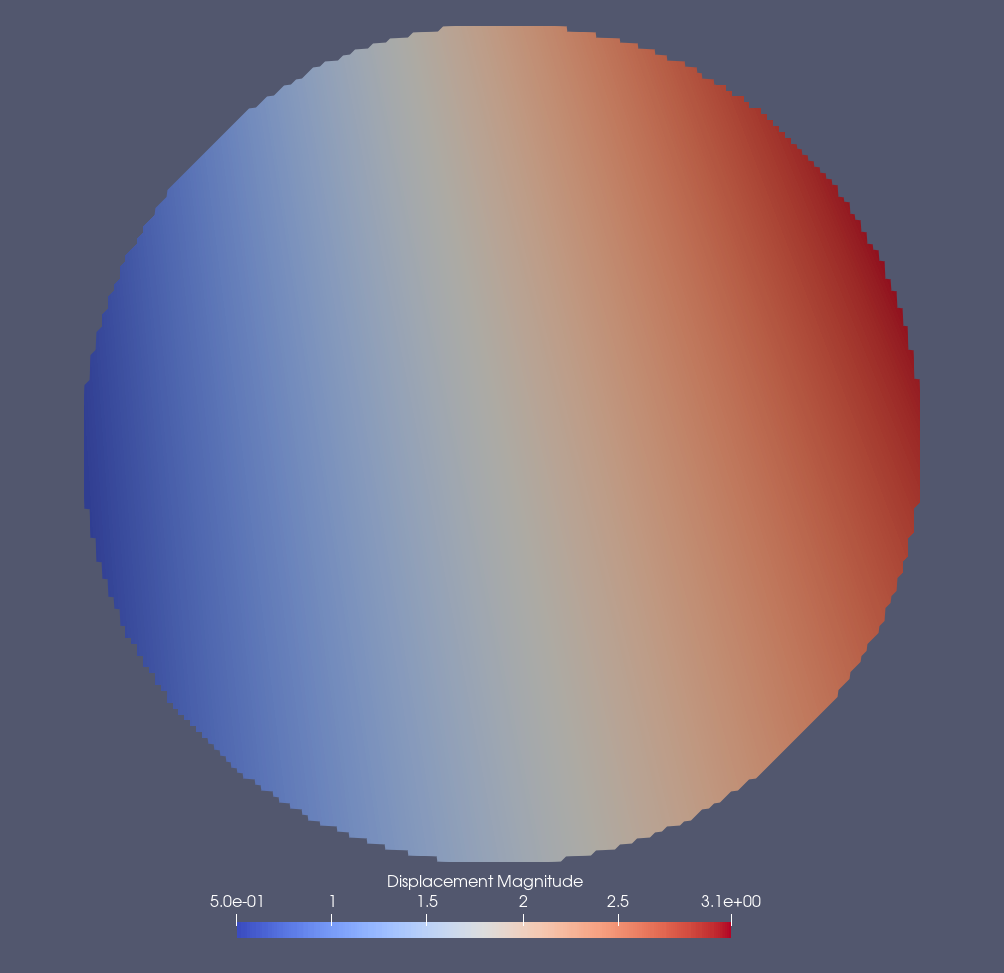
\includegraphics[width=\textwidth]{StabElasPara1.png}
        \caption{Solution's magnitude in Paraview}
        \label{fig:Para3}
    \end{subfigure}
    % \hfill
    \begin{subfigure}[b]{0.50\textwidth}
        % \centering
        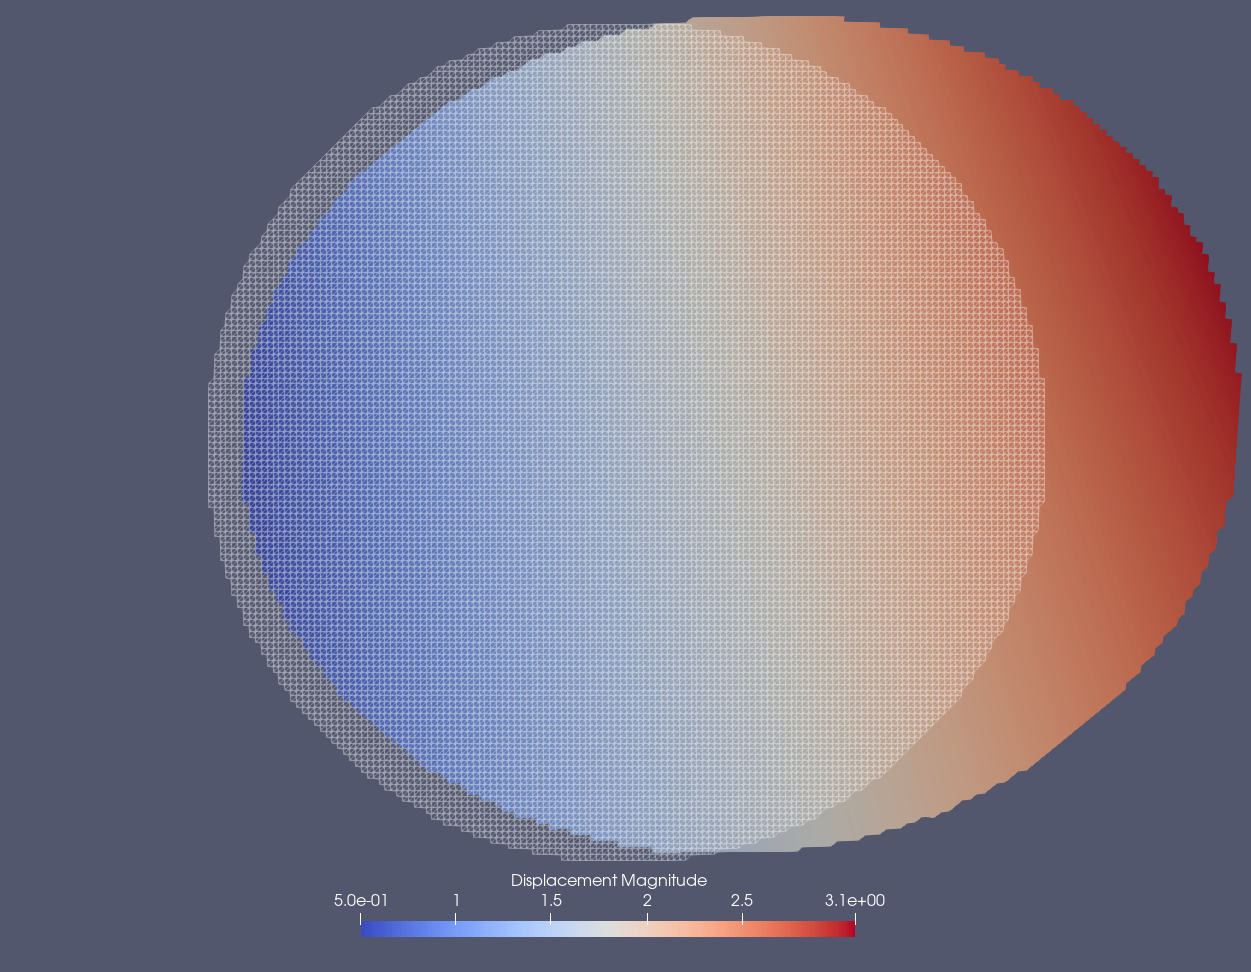
\includegraphics[width=\textwidth]{StabElasPara2.png}
        \caption{Solution warped by vector in Paraview}
        \label{fig:Para3}
    \end{subfigure}
    \begin{subfigure}[b]{0.45\textwidth}
        % \centering
        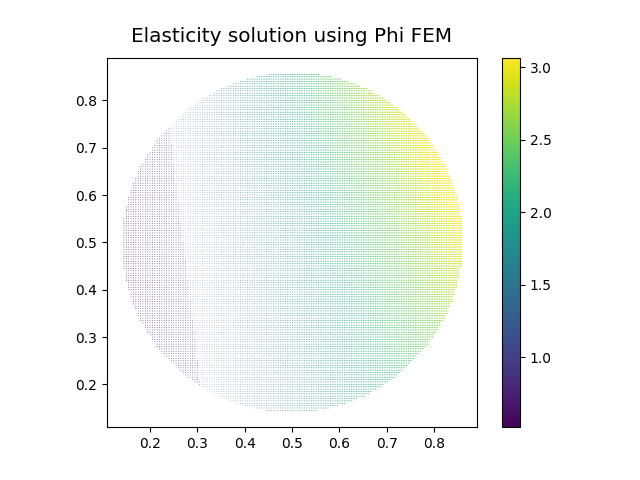
\includegraphics[width=\textwidth]{StabElasSol.png}
        \caption{Solution's components (vector) in Matplotlib}
        \label{fig:StabElasSol}
    \end{subfigure}
    % \hfill
    \begin{subfigure}[b]{0.45\textwidth}
        % \centering
        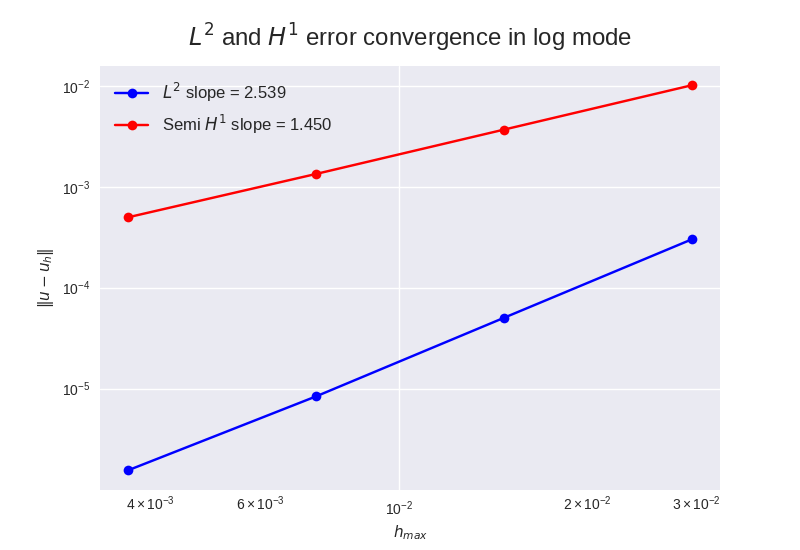
\includegraphics[width=\textwidth]{StabElasCvg.png}
        \caption{Convergence study}
        \label{fig:StabElasCvg}
    \end{subfigure}
    % \hfill
       \caption{Results obtained when applying the \phifem  technique to the elasticity equation \eqref{eq:elasticity}. The convergence study in done with relative errors. The $H^1$ slope indicated in (D) is the $H^1$ semi-norm $ | u - u_h|_{1, \Omega\cap\Omega_h}$.}
       \label{fig:StabElas}
\end{figure}


\section{Results summary}

The table \ref{tab:results1} and the figure \ref{fig:results2} below summarize the results we obtained. All the errors that are presented are relative errors. We used the $H^1$ norm for the Poisson problem, and the semi-$H^1$ norm for the elasticity equation. We can see that for each of the problems we solved, the \phifem approach was better than the standard FEM approach.

\begin{table}[h!]
    \centering
    \begin{tabular}{c| l| c| c}
        \toprule
        \tabhead{Problem} & \tabhead{Technique} & \tabhead{$L^2$ slope} & \tabhead{$H^1$ slope} \\
        \midrule
        \multirow{2}{4em}{Poisson} & Classic FEM & 2.041 & 1.013 \\
         & \phifem & 2.550 & 1.461 \\
        \midrule
        \multirow{2}{4em}{Elasticity} & Classic FEM & 1.971 & 0.974 \\
         & \phifem & 2.539 & 1.450 \\
        \bottomrule
    \end{tabular}
    \caption{Data summarizing the convergence results.}
    \label{tab:results1}
  \end{table}


  \begin{figure}[H]
    \centering
    \begin{subfigure}[b]{0.45\textwidth}
        % \centering
        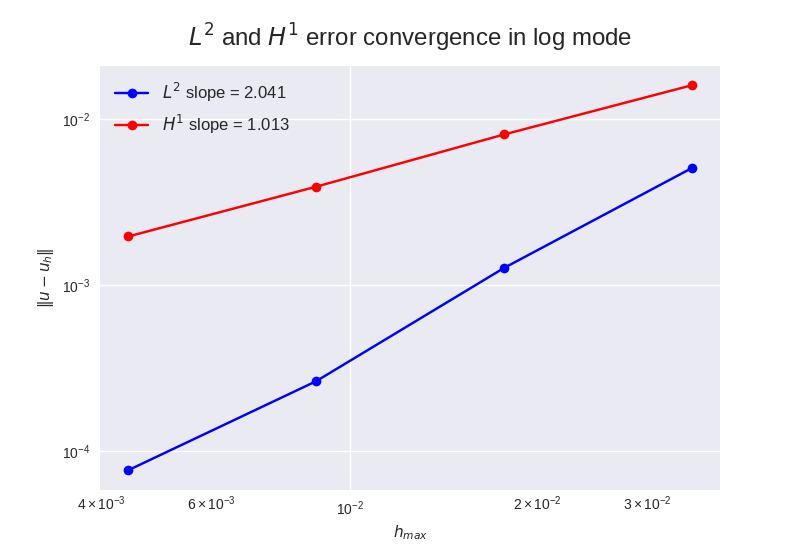
\includegraphics[width=\textwidth]{ClassicCvgStudy2.png}
        \caption{Poisson using Classic FEM}
    \end{subfigure}
    % \hfill
    \begin{subfigure}[b]{0.45\textwidth}
        % \centering
        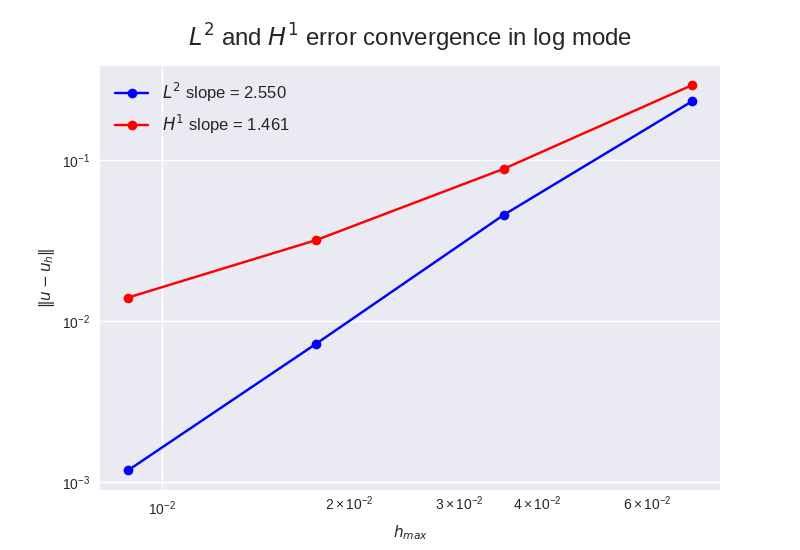
\includegraphics[width=\textwidth]{StabCvgStudy.png}
        \caption{Poisson using \phifem}
    \end{subfigure}
    \begin{subfigure}[b]{0.45\textwidth}
        % \centering
        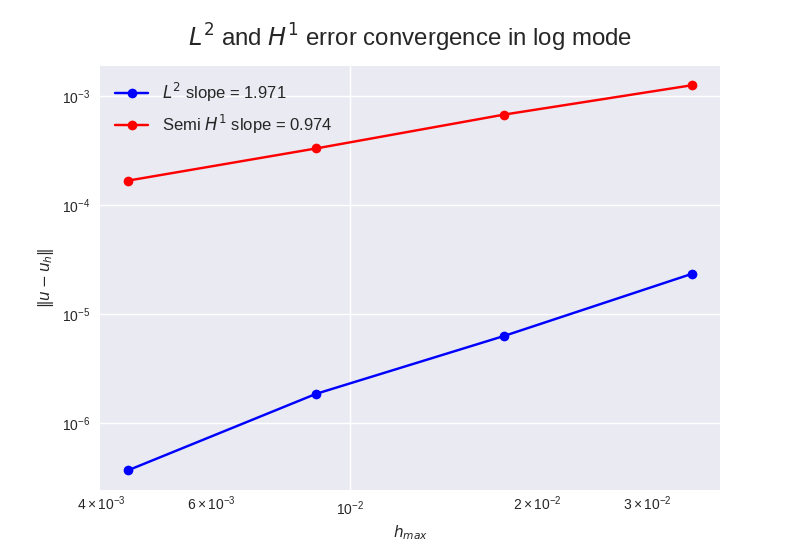
\includegraphics[width=\textwidth]{ClassicElasCvg.png}
        \caption{Elasticity using Classic FEM}
    \end{subfigure}
    % \hfill
    \begin{subfigure}[b]{0.45\textwidth}
        % \centering
        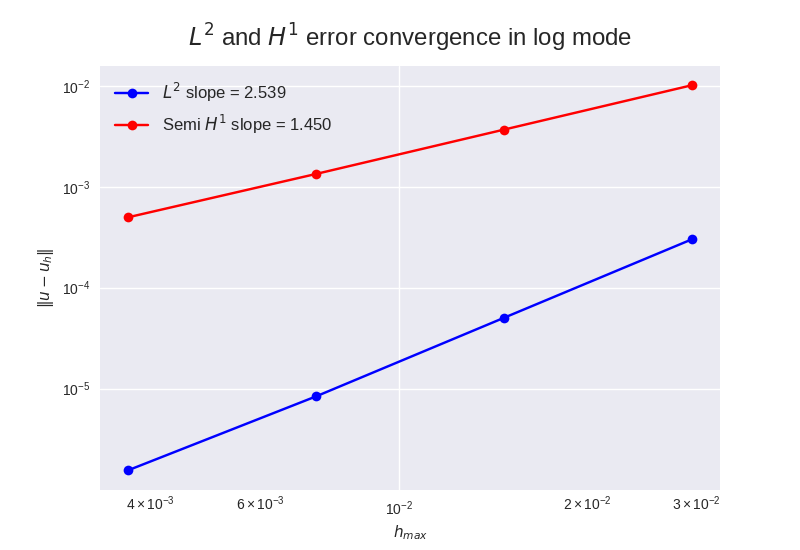
\includegraphics[width=\textwidth]{StabElasCvg.png}
        \caption{Elasticity using \phifem}
    \end{subfigure}
    % \hfill
       \caption{Comparison of the convergence results we obtained from the previous sections.}
       \label{fig:results2}
\end{figure}
